\documentclass{GlobalDocument}
\usepackage[landscape, top=0.5in, bottom=0.5in, left=2in, right=0.3in]{geometry}
\usepackage{subcaption} % for sub-figures
\usepackage{array}
\usepackage{pdfpages}
\usepackage{multirow}
\usepackage{multicol}
\usepackage{wrapfig}

\usepackage{float}

\begin{document}
% Title Page
\title{Design Document}
\author{\ourteam}

%\maketitle
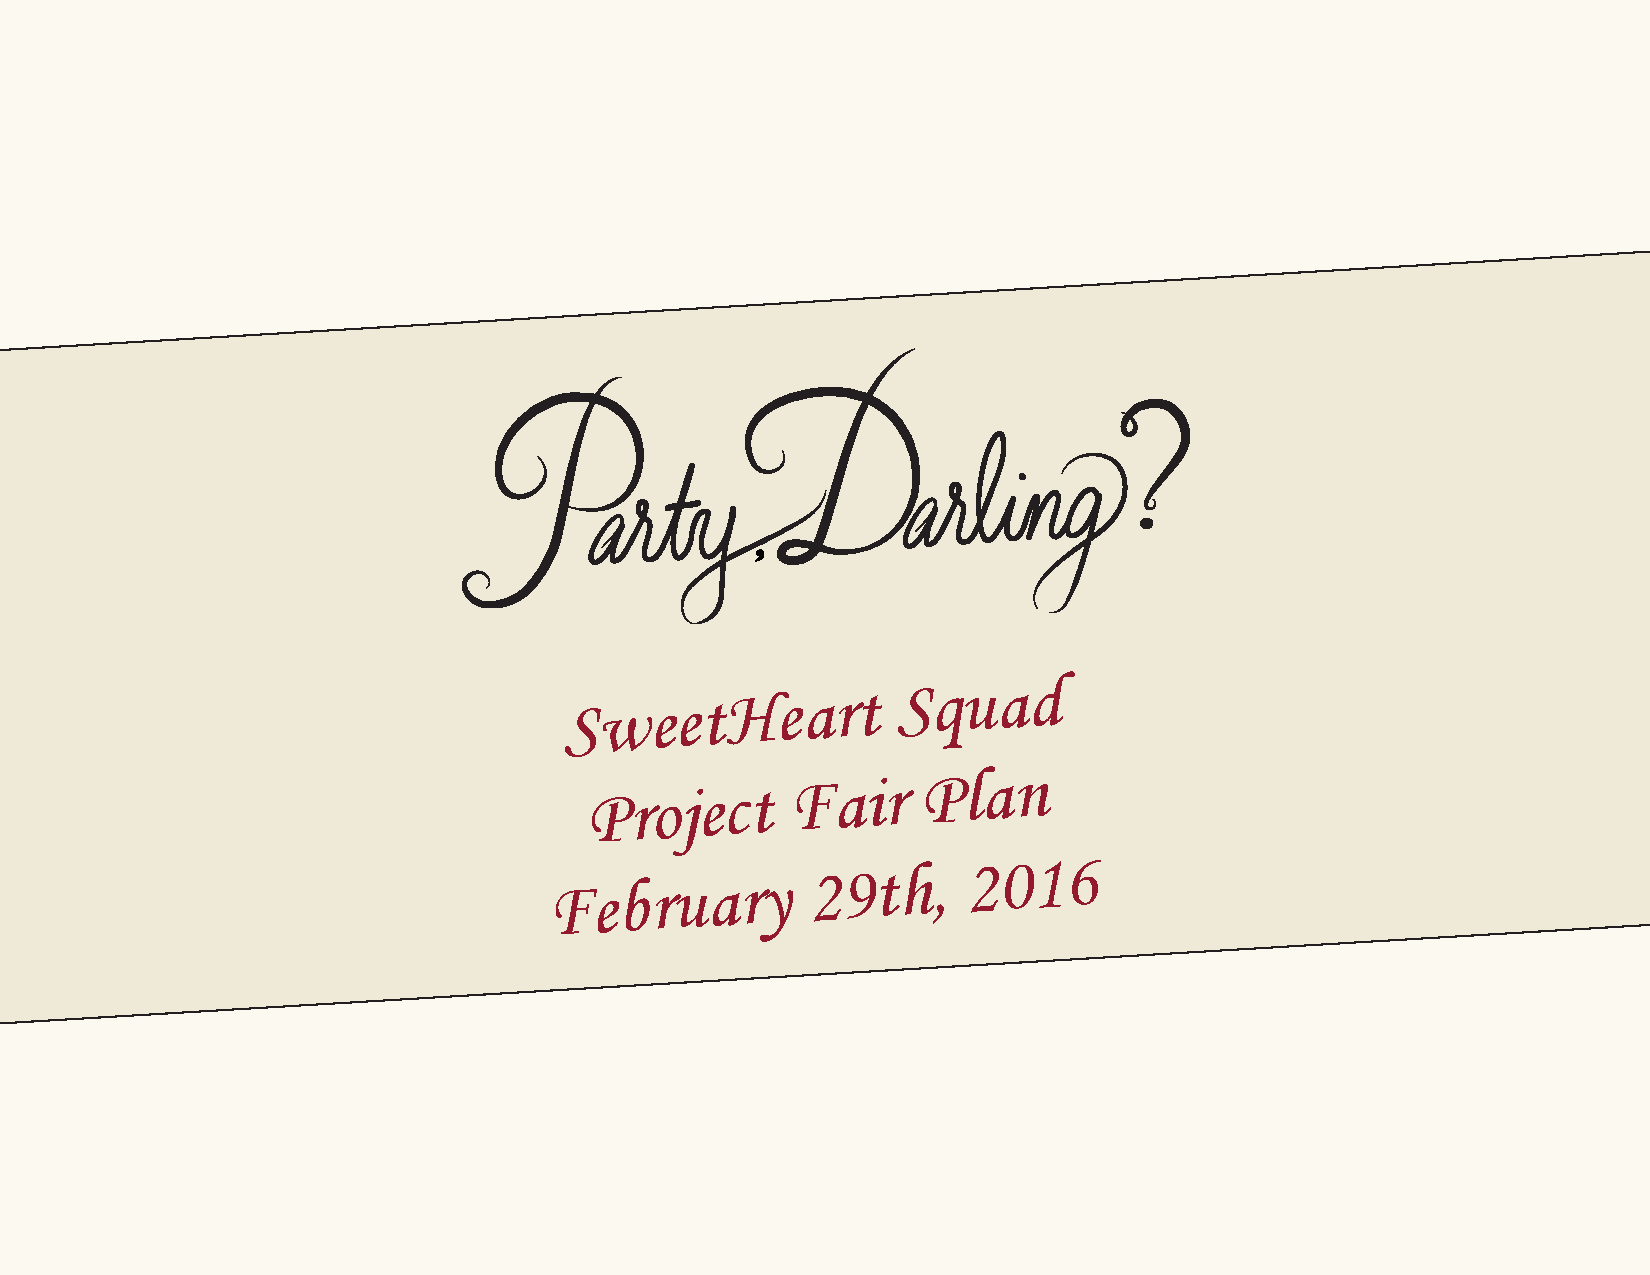
\includepdf{TitlePage}

\BgUsetrue % activates background (leave this off while working, it makes the compilation waaay slower)

\chapter{Layout}
The room intended for \ourteam{}'s use during the fair is AP132. The intended layout can be seen in Figure~\ref{fig:layout}. As there are 6 senior project groups and limited space, it is possible that the room will be shared by \ourteam{} and another group. To prepare for this, the room layout has been designed based on the assumption that it will minimally be designated half the room, with the potential to mirror to the other side.

\begin{figure}[htb]
	\centering
	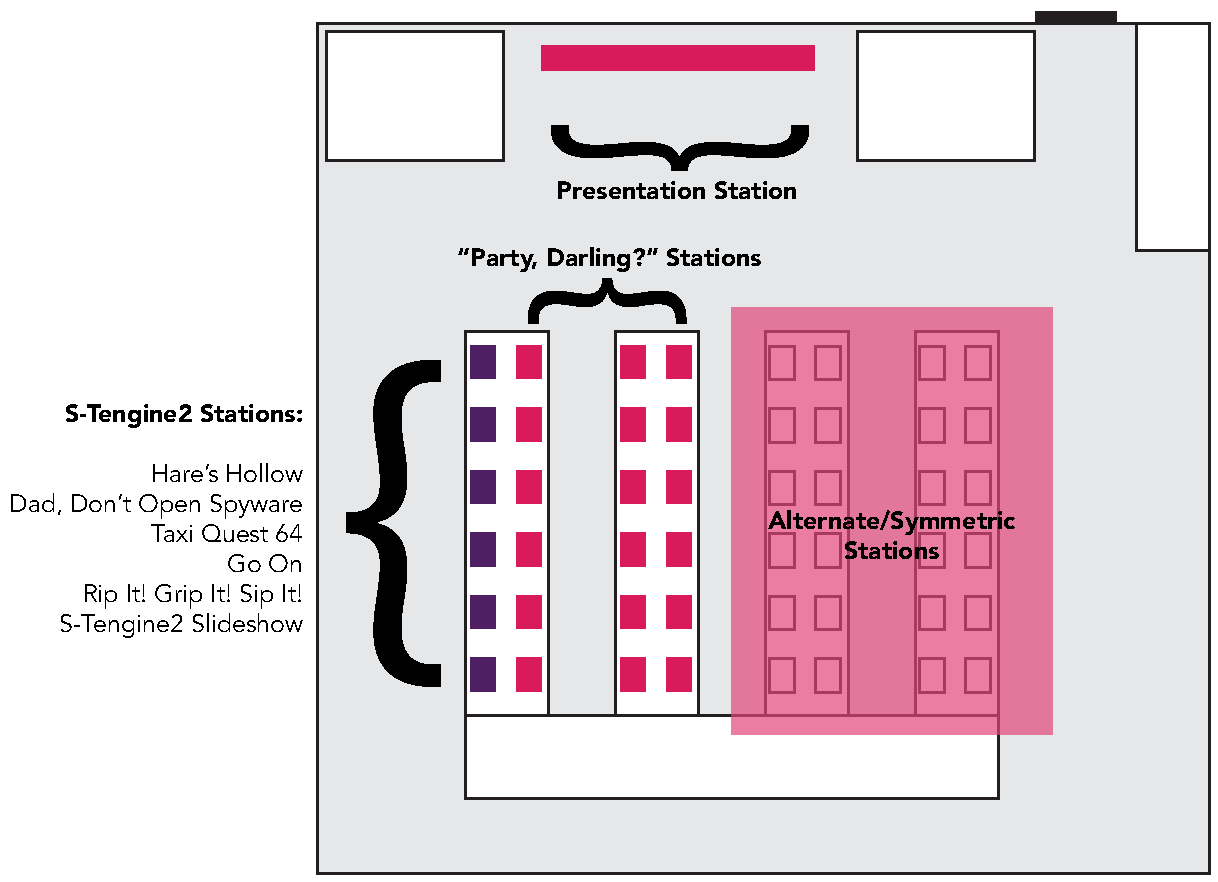
\includegraphics[width=\textwidth]{images/layout}
	\caption{AP132 Room layout}
	\label{fig:layout}
\end{figure}

\section{Presentation Station}
The front of the room will be converted into the main presentation area by moving the center table out of the way and including a large screen television connected to a team member's laptop.

\section{\ourgame{} Stations}
Of the four rows of computers in the layout, the three closest to the center will be reserved as stations for \ourgame{}. Earbuds/headphones will be required for each station. No additional software will be required, as the game can be installed simply by extracting a zip archive onto each computer's desktop.

\section{\ourengine{} Stations}
In addition to the main feature, \ourgame{}, we intend to highlight the development of \ourengine{} during the fair. The furthest set of stations will show other products created using \ourengine{} during the term of senior project in chronological order - these are listed in Figure~\ref{table:products}. Each station will be accompanied by a small poster (laminated and taped to the table) which summarize the engine's progress at the time of development. These stations will similarly require earbuds/headphones, but no additional software.

In addition to the five products listed in Figure~\ref{table:products}, a sixth station will be setup at the end of the row which has a looping multimedia presentation, showing screenshots, animated gifs, etc. from \ourengine{} products\footnote{This may include media from smaller projects which were excluded from the fair stations.}.
%SweetBeats & ProcJam & 2015-11-15 & fbg\\ \hline
%Super Spaceship 64 & Mini-Ludum Dare 64 & 2016-01-24 & fbg\\ \hline

\chapter{Decorations}

\section{Posters}
\subsection{Development Posters}
In order to highlight certain aspects of \ourgame{}, \ourengine{}, and our development process we will be placing additional posters on the walls of our room.

\begin{figure}[htb]
	\centering
	\begin{tabular}{ | p{7cm} | p{7cm} |}
		\hline
		Title & Description \\ \hline
		
		\textit{Character Concept Poster}&
		This poster will show the various styles proposed for the characters of our game before starting development.\\ \hline
		
		\textit{Early Room Concept Poster}&
		This poster will show the concept art of a room in Party Darling, created at the beginning of development\\ \hline
		
		\textit{Engine Timeline Poster}&
		This poster will be used to show the various stages of development of our custom engine, STengine-2. It will detail key milestones, features, and games created with the engine.\\ \hline
		
		\textit{Room Generation Poster}&
		This poster will detail the various steps involved with room generation, including creating the room layout, generating the room mesh, and placing furniture.\\ \hline
		
		\textit{Furniture Generation Poster} &
		This poster will detail the steps used to create the generative furniture within Party Darling, using a single type of furniture as an example.\\ \hline
		
		\textit{Character Generation Poster} &
		This poster will detail the steps used to create the generative furniture within Party Darling, using a single type of furniture as an example.\\ \hline
		
	\end{tabular}
	\caption{Descriptions of the posters which we will include in our presentation room}
	\label{table:products}
\end{figure}

\subsection{\ourgame{} Posters}
In order to highlight certain aspects of \ourgame{}, we will be placing additional posters on the walls of our room. One poster will include every character created during the design phase of the project, arranged in a "Where's Waldo" style layout. Another will show four screenshots of in-game procedurally generated rooms, showing the variety of furniture and layouts possible.

\subsection{\ourengine{} Posters}
In order to highlight the effort that went into the development of \ourengine{} during the senior project term, we will also be placing posters related to the engine on the walls of our room. One poster will include a timeline of the engine's development with major releases marked. Another will show a rough engine architecture diagram, showing the different layers of engine code and the interaction between \ourteam{}'s development and the open-source libraries upon which \ourengine{} is built. For a list of which projects we will be creating posters for, please see Figure ~\ref{fig:st_products}.

\begin{figure}[htb]
\centering
    \begin{tabular}{ | p{3cm} | p{3cm} | c | p{5.5cm} | p{6cm} |}
    \hline
    Title & Source & Release & Game Summary & Engine Progress \\ \hline
    
    \textit{Hare's Hollow}&
    Write A Game Challenge&
    Jun 6th, 2015&
    An exciting visual novel for 3 of your 5 senses. Play as Fox and explore Hare's Hollow to discover the secret story of the animals.&
    The first game to be produced during senior project, \textit{Hare's Hollow} was intentionally designed to require a complete UI layout system and a sophisticated dialogue parser with support for triggering branching conversations and triggering events.\\ \hline
    
    \textit{Dad, Don't Open Spyware}&
    Ottawa Game Jam&
    Jul 2nd, 2015&
    This is a game of coordination. As a Mother/Son hacker team, you must press your special attack buttons at the same time to initiate powerful moves. Don't be a victim of bad data -- defeat waves of viruses and net nasties to save the day!&
    In addition to adding controller support, \textit{Dad, Don't Open Spyware} helped to stress-test the asset management system in \ourengine{}. Since the game was developed in a mere 48 hours (to contrast, WAG Challenge was a full month), it also helped to assess the speed of \ourteam{}'s pipelines.\\ \hline
    
    \textit{Taxi Quest 64}&
    Ludum Dare 34 &
    Dec 14th, 2015&
    A short narrative experiment.&
    Made to ensure that the recently-updated dialogue system was stable, \textit{Taxi Quest 64} used random scenario selection routine similar to \ourgame{}'s.\\ \hline
        
    \textit{Go On}&
    Ludum Dare 34&
    Dec 14th, 2015&
    A two-button game about growing up.&
    Like \textit{Taxi Quest 64}, this was made to test out new/updated features. During development, several issues with the lighting model were identified and solved.\\ \hline
    
    \textit{Rip It! Grip It! Sip It}! &
    Global Game Jam&
    Feb 3rd, 2016&
    Father Skyler has been hired to exorcise some demons running rampant at the local country club. Can he save everyone in time? Will he get arrested again for his wild card tendencies? Play the game to find out! &
    At this point during development, \ourengine{} was feature-complete and free of any known major bugs. The relatively painless development of \textit{Rip It! Grip It! Sip It!} served as a testament to the progress made throughout the term.\\ \hline
    
    \end{tabular}
\caption{\ourengine{} products (with summaries and engine contributions) to be shown during fair}
\label{fig:st_products}
\end{figure}

\section{Cardboard Cutout}
A life-sized cardboard cutout of one of our designed characters will be made to decorate the presentation space. It will have elbow and shoulder joints to allow for arm movement. 

The room will also be populated with smaller cardboard cutouts of characters. These characters will be placed beside computers and on the tables in the room. Please see Figure~\ref{fig:cutout} for an image of a prototype cutout.

\begin{figure}[htb]
	\centering\begin{subfigure}{.45\textwidth}
	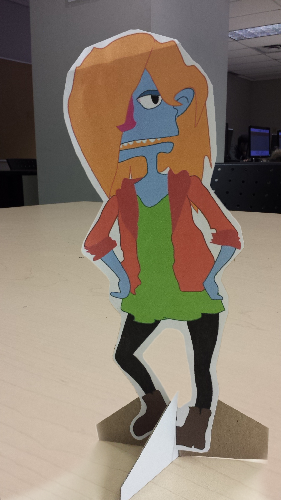
\includegraphics{images/cutout}
	\end{subfigure}
	\caption{Prototype cardboard cutout}
	\label{fig:cutout}
\end{figure}

\chapter{Additional Materials}
\section{Chocolate}
To show what a bunch of sweethearts the members of \ourteam{} are, the team plans to provide our guests with chocolate hearts. The chocolate will be placed on one of the tables provided in the presentation room.

\section{Business Cards}
For networking purposes, each member will be printing a business card to represent themselves. The cards will be placed on one of the tables provided in the presentation room.
\end{document}